\FloatBarrier
\begin{figure}[!h]
\centering
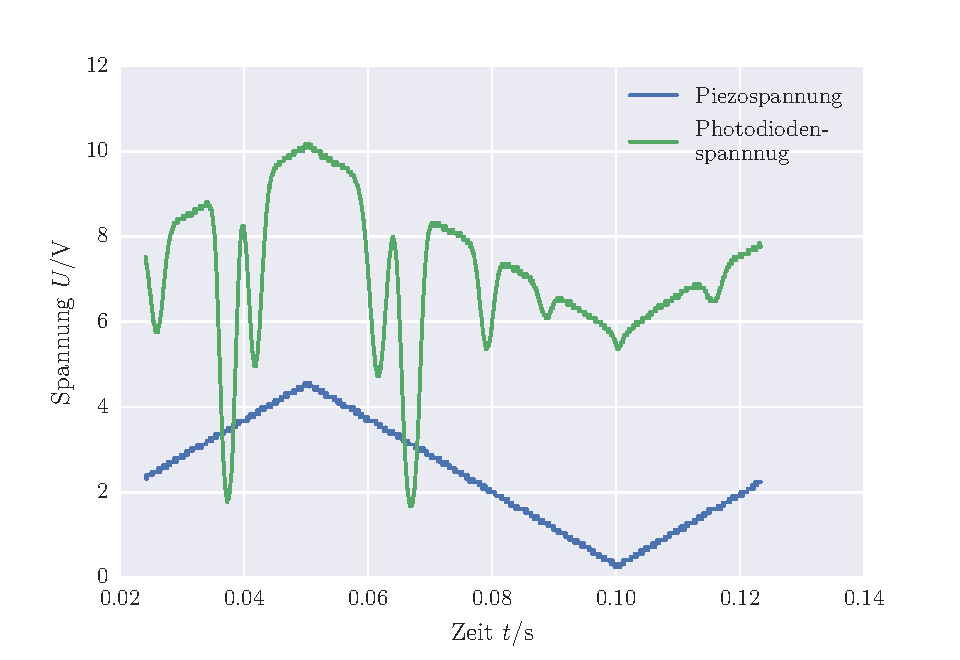
\includegraphics[scale=1]{../Grafiken/Strommodulation.pdf}
\caption{Spannungsverläufe der zu Modulation von Piezo und Strom verwendeten 
	Dreieckspannug und dem Signal der Photodiode. Das Abfallen der hier im Vergleich
	zu vorher invertierten Photodiodenspannung ist die Folge der Strommodulation.
	Es ist jedoch schon erkennbar das durch die Strommodulation keine Modensprünge 
	mehr auftreten.
	\label{fig:strommodulation}}
\end{figure}
\FloatBarrier